\documentclass[article]{uom-coursework}

\usepackage{blindtext}
\usepackage[showframe]{geometry}
\usepackage{float}


\counterwithout{section}{chapter}

% Biblography
% \addbibresource{dsa.bib}

\title{Data Structures and\\Algorithms 2}
\tagline{Coursework}
\author{Juan Scerri}
\authorid{1234567A}
\courseworkname{Some Degree}
\doctype{coursework}
\courseworkdate{\monthyeardate\today}
\subjectcode{ICS2210}


\begin{document}

%----------------------------------
%	Front Matter
%----------------------------------

\pagestyle{umpage}

\frontmatter

\maketitle % Print the title page

\tableofcontents % Print the table of contents

\clearpage

\lstlistoflistings

\clearpage

\mainmatter

% \chapter{Report}

\chapter*{Report}
\label{chap:report}
\addcontentsline{toc}{chapter}{\nameref{chap:report}}

% TODO: the report
% add reason for language
% add comments for explanation
% add lstlisting describing the knuth_shuffle
% add lstlisting describing the untyped_tree
% add lstlisting describing the untyped_avl_tree
% add lstlisting describing the untyped_rb_tree
% add lstlisting describing the skip_list
% then explain the procedure.py and what is does
% add a section describing the statistics

\section{Language}

The programming language used for this coursework is Python 3.
The main reason for this choice is the speed of development.

\section{Comments}

Throughout the code an effort was made to deliver explanations
through comments. In Python comments start with a \#. Moreover,
in the listings comments have a grey colour.

\section{Knuth Shuffling}

\lstinputlisting[caption={A function implementing Knuth shuffling.},language=Python,firstline=8,lastline=13]{../ics2210/knuth_shuffling.py}

Knuth shuffling, also known as Fisher--Yates shuffling, is an
algorithm used for generating permutations of the elements of a
given array.

The implementation follows the pseudocode described here:
\url{https://en.wikipedia.org/wiki/Fisher%E2%80%93Yates_shuffle#The_modern_algorithm}

\section{Binary Search Tree}

A decision was made to first implement a Binary Search Tree
(BST) because the basic structure of a BST is underlying both
AVL and Red-Black trees, helping reduce code duplication.

The file \texttt{untyped\_tree.py} contains two of our base
building blocks. In particular these are \texttt{Node} and
\texttt{Tree}. As described the \texttt{Tree} class is a BST
with the main method being \texttt{insert()}. This is a basic
BST insert. Note however that a number of
methods associated with the Node class are being
used.

Additionally, when creating a tree one
can enable statistics and keep track of the
number of steps for insertion to complete.

Additional methods required for collecting certain
statistics are: \texttt{calc\_height()} and
\texttt{calc\_leaves()}. They are
quite self-explanatory, one is used to calculate
the height of the tree whilst
the other is meant to calculate the number of
leaves the tree has.

In particular these methods are recursive in
nature. Although the trees we are
using are balanced and hence cannot
exhibit the worst-case scenario in terms
of height which an unbalanced BST tree can,
it is still possible for sufficiently large
trees to exceed the recursion limit of
the language in use. Note however,
for the number of elements that are being
tested this is more than sufficient.

Finally, I would like to draw your attention
to the \texttt{draw()} method which
was invaluable during the development of
such algorithms to ensure that the implemetation
is in parity with other impelemetations.

If you wish to test the implementations for
yourself please either use \texttt{python}
or \texttt{ipython}. Additionally, please ensure
that you are in the root directory of the project.
Then follow the commans in TODO FIGURE

The simplest idea here is that we get to make us

\begin{figure}[H]
\centering
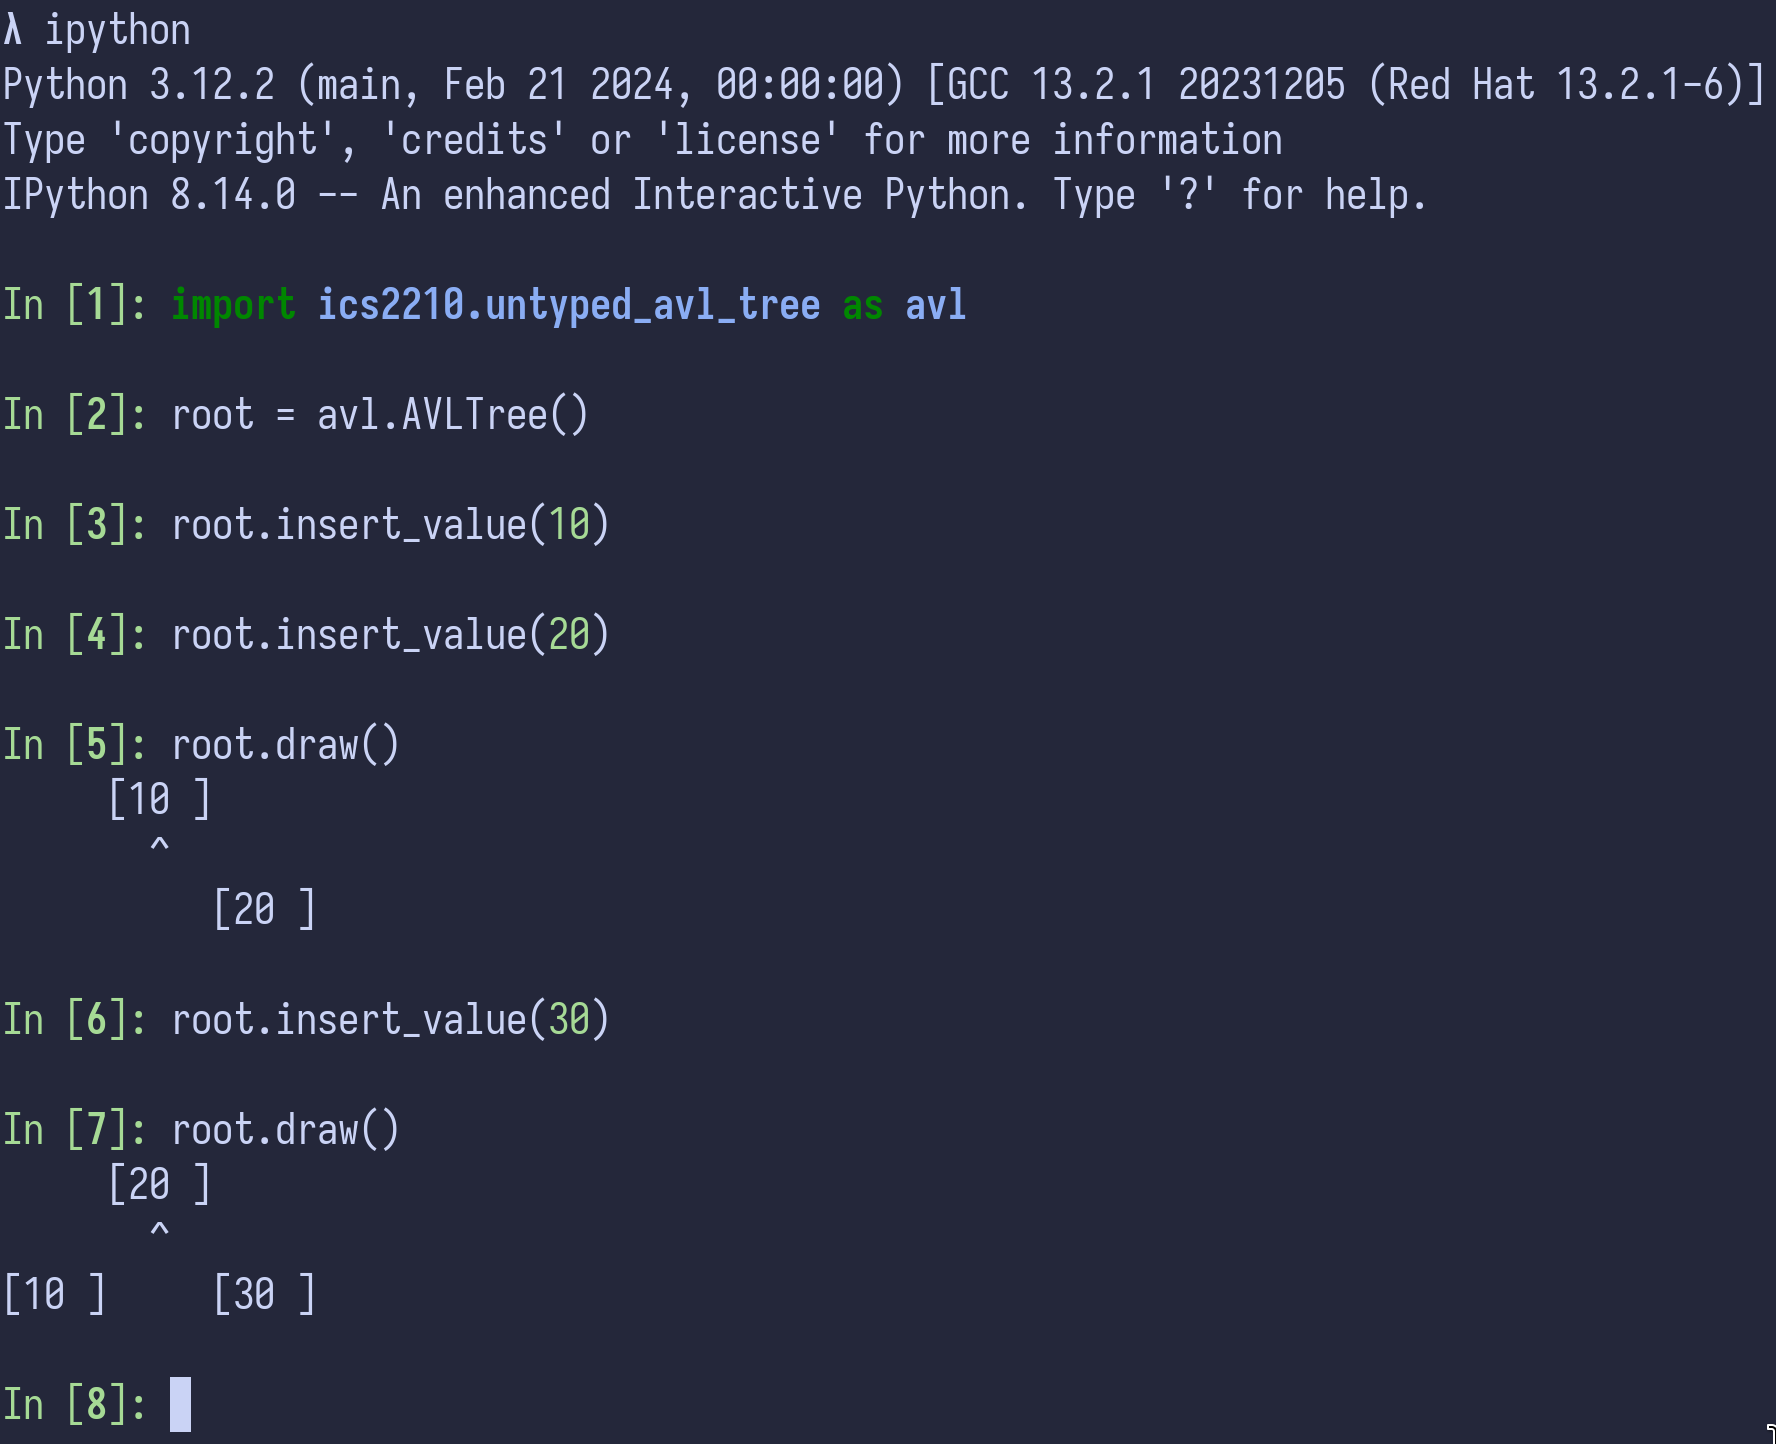
\includegraphics[width=\linewidth]{using-ipython-avltree.png}
\caption{An image of using an AVLTree (similar interface for an RBTree).}
\label{fig:test9}
\end{figure}

\begin{figure}[H]
\centering
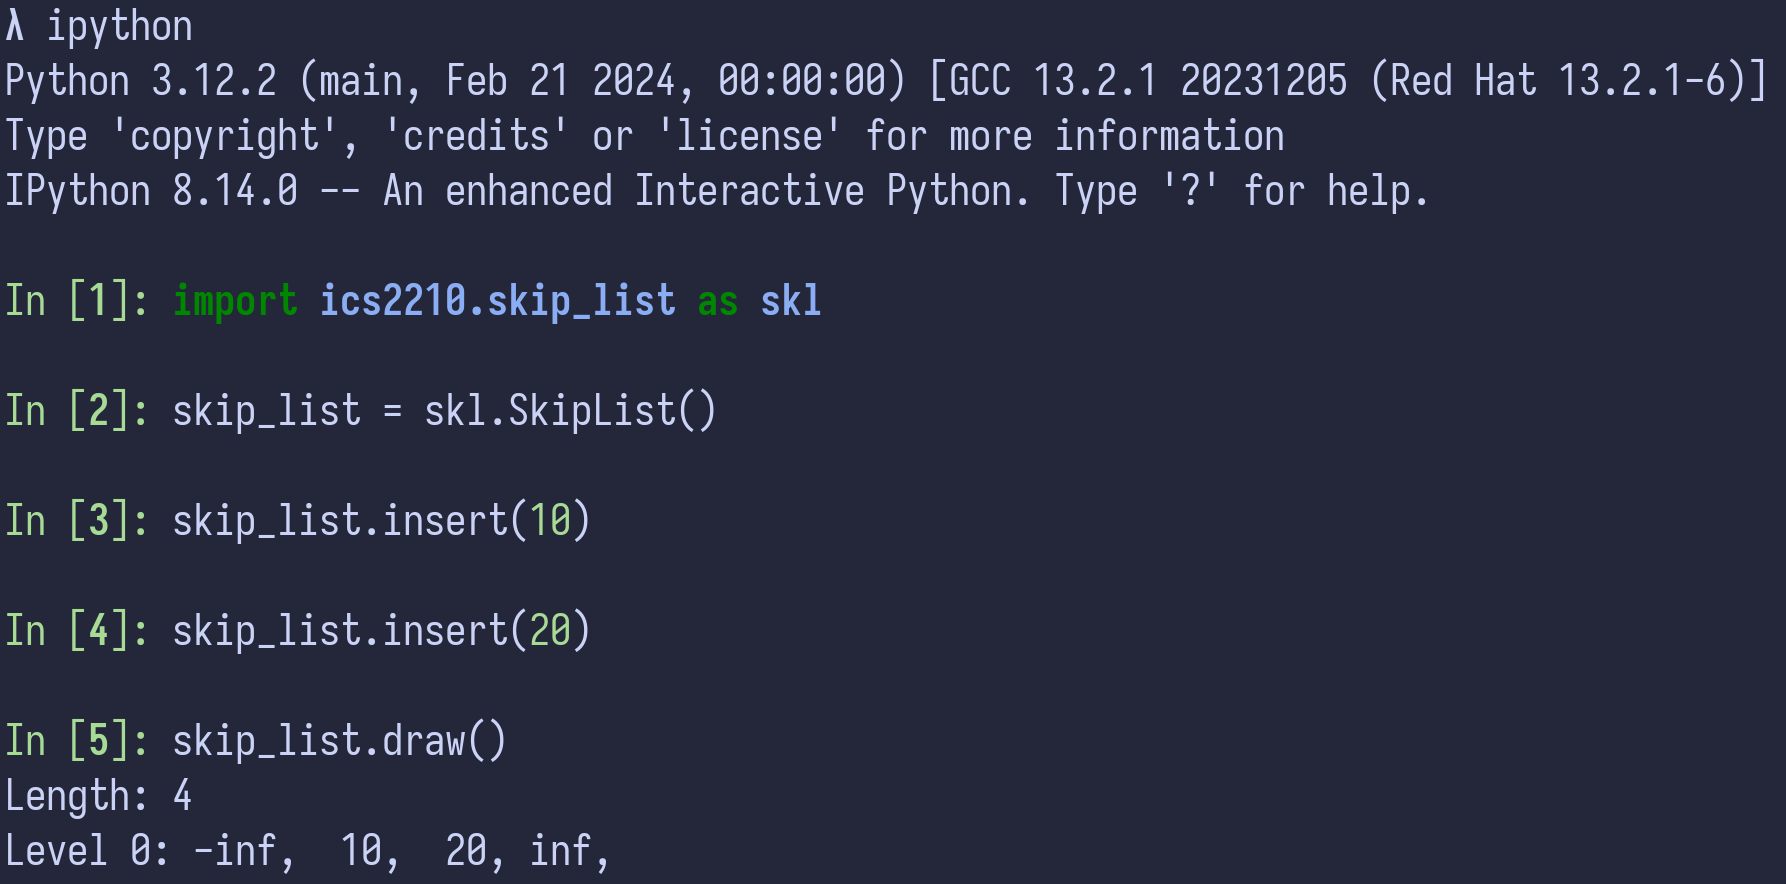
\includegraphics[width=\linewidth]{using-ipython-skiplist.png}
\caption{An image of using an AVLTree (similar interface for an RBTree).}
\label{fig:test9}
\end{figure}

Additionally, they have a baked in example which
can be run to test the behvaiour of data structures.

\begin{figure}[H]
\centering
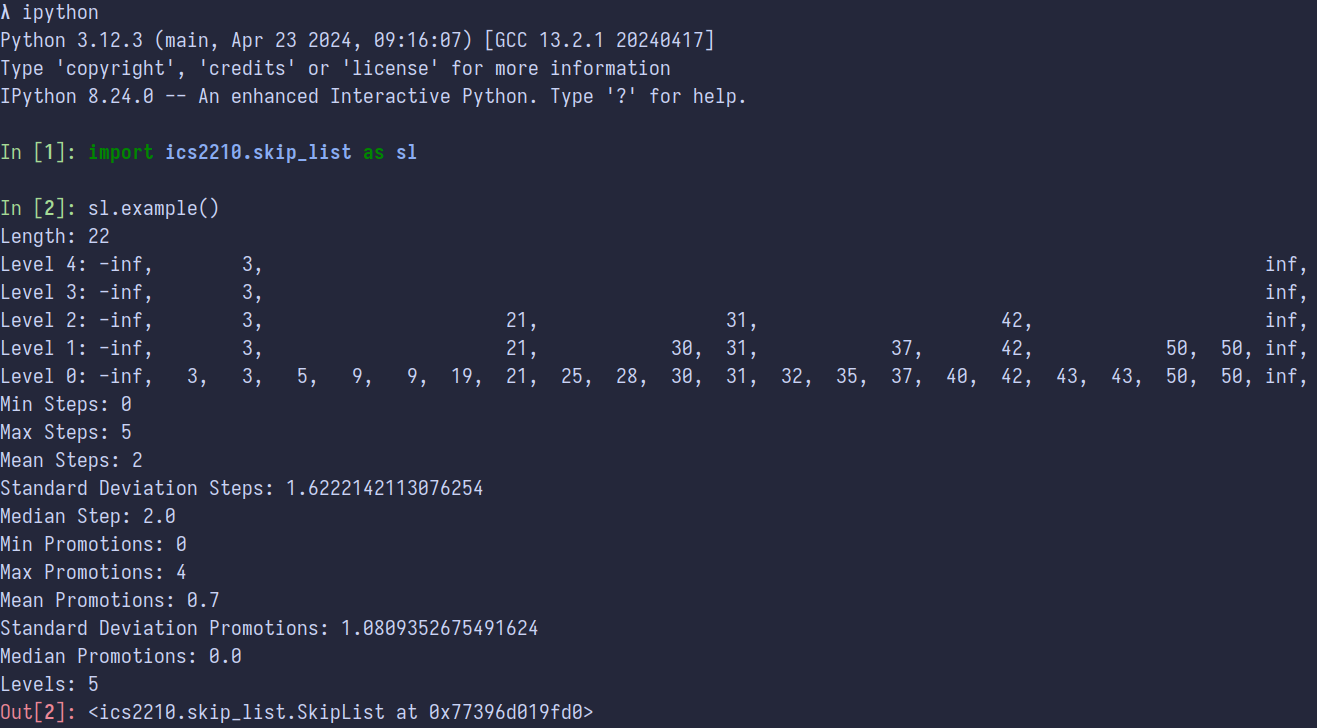
\includegraphics[width=\linewidth]{ipython-skiplist-example.png}
\caption{An image using the builtin an SkipList example with statistics (similar interfaces for an AVLTrees RBTrees are present).}
\label{fig:test9}
\end{figure}

Now I would like to discuss the Node class which is
a bit more complicated then a pure Node. A
variety of methods which help facilitate 
and maintain readable code with in the
complete data structures is present
here.

In particular, the following methods
\texttt{rotate()}, \texttt{can\_step()},
\texttt{value_dir()} and \texttt{dir()}.
The other methods present I believe are
very self explanatory.

\texttt{can\_step()} method
returns a boolean allowing us to know whether or not
a node has a child in the specified direction.

\texttt{value\_dir()} accepts a value, of course the value has
to be comparable with the element present in the node. Then
depending on whether the value is greater than or less than the
the value in the node a direction will be provided. In
particular, if its is less than, the LEFT direction will be
provided and if it is greater than or equal to the RIGHT
direction is provided.

\texttt{dir()} is used to check wheter an other
node is on the left or right of the current node
(of course the current node is the node referenced
as self.) NOTE: this method is unsafe
in the sense that if a other node
is provided and it is not a child the
self node then it will be classified as being
on the right of the node which is of course
incorrect.


\texttt{rotate()} finally the rotate
method is a generalized ll or rr
rotation method. Note that lr and
rl can be achieved by using combinations
of ll and rr.

Additionally, this rotate method has been heavily
inspired by the rotate method used on
wikipedia for the implementation
of red-black trees.

In particular,

\section{Section?}
\section{Section?}
\section{Section?}
\section{Section?}
\section{Section?}
\section{Section?}
\section{Section?}
\section{Section?}


\blindtext
\blindtext
\blindtext

\end{document}
